\subsection{External interface requirements}
\subsubsection{User interface}

\begin{figure}[!h]
	\centering
	\begin{minipage}[b]{0.65\textwidth}
		\makebox[\textwidth][c]{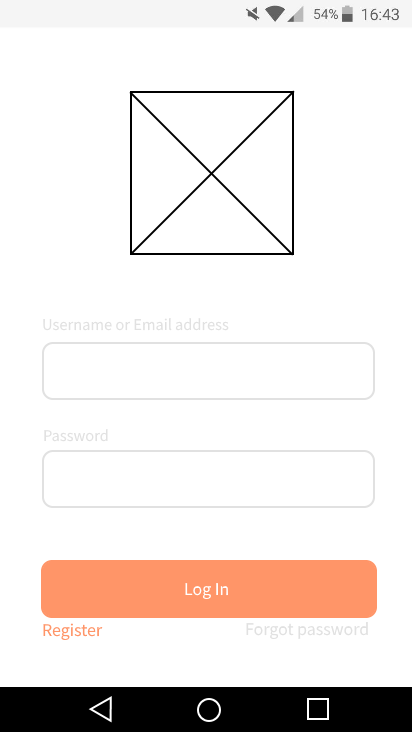
\includegraphics[width=0.50\textwidth]{Images/Mockup/LogPage.png}}%
		\caption{Login page}
	\end{minipage}
	\begin{minipage}[b]{0.65\textwidth}
		\makebox[\textwidth][c]{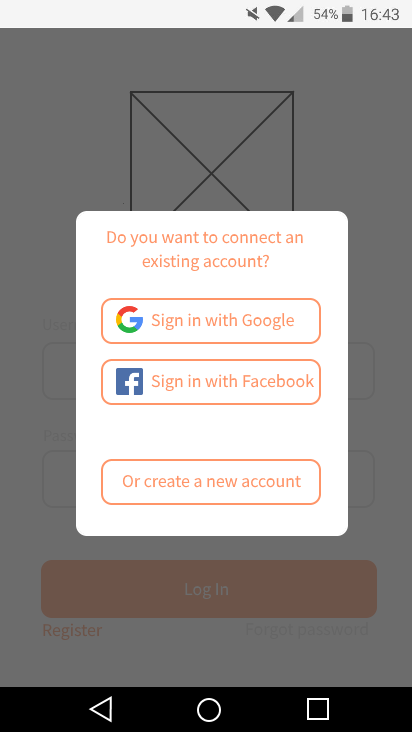
\includegraphics[width=0.50\textwidth]{Images/Mockup/GoogleConnectionPopup.png}}%
		\caption{Connection of an existent account}
	\end{minipage}
\end{figure}
\clearpage
\begin{figure}[!h]
	\centering
	\begin{minipage}[b]{0.65\textwidth}
		\makebox[\textwidth][c]{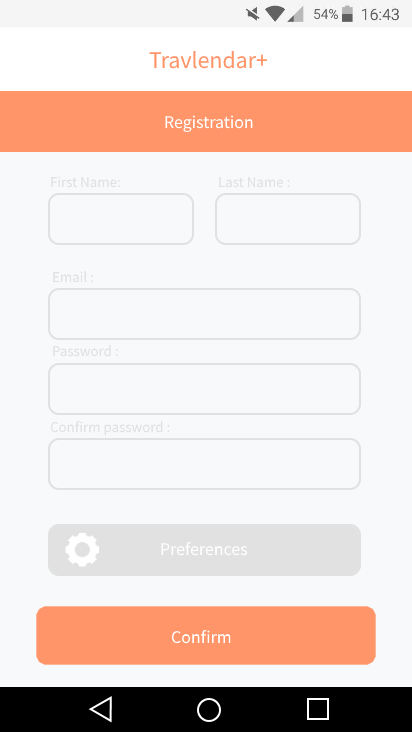
\includegraphics[width=0.50\textwidth]{Images/Mockup/RegistrationForm.png}}%
		\caption{Registration form}
	\end{minipage}
	\begin{minipage}[b]{0.65\textwidth}
		\makebox[\textwidth][c]{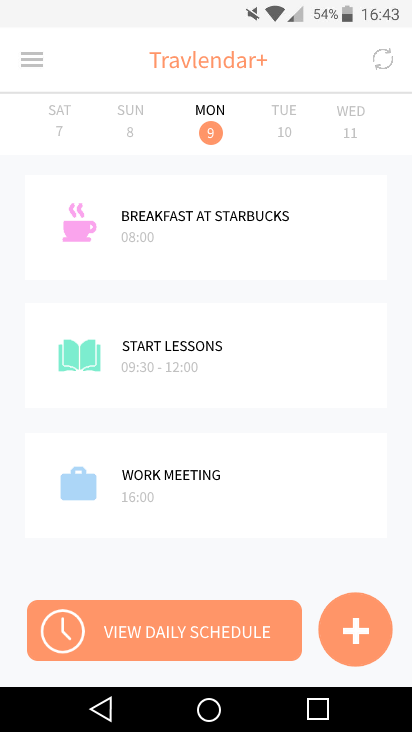
\includegraphics[width=0.50\textwidth]{Images/Mockup/Base.png}}%
		\caption{Daily view of calendar}
	\end{minipage}
\end{figure}
\clearpage
\begin{figure}[!h]
	\centering
	\begin{minipage}[b]{0.65\textwidth}
		\makebox[\textwidth][c]{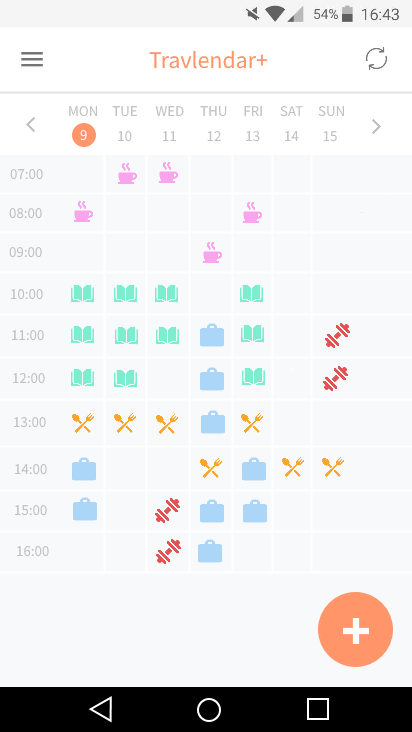
\includegraphics[width=0.50\textwidth]{Images/Mockup/Base3.png}}%
		\caption{Weekly view of calendar}
	\end{minipage}
	\begin{minipage}[b]{0.65\textwidth}
		\makebox[\textwidth][c]{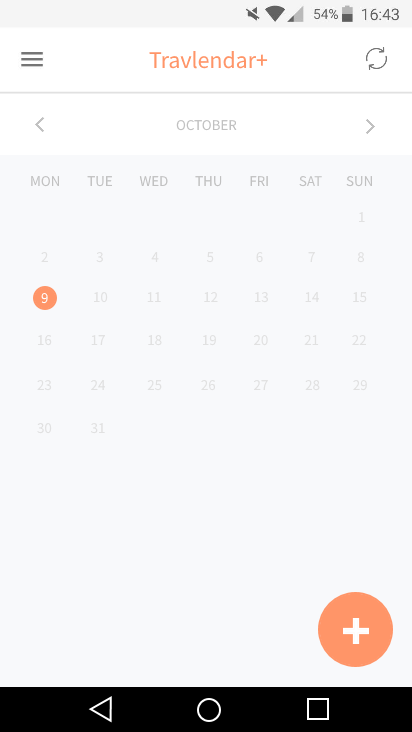
\includegraphics[width=0.50\textwidth]{Images/Mockup/Base2.png}}%
		\caption{Monthly view of calendar}
	\end{minipage}
\end{figure}
\clearpage
\begin{figure}[!h]
	\centering
	\begin{minipage}[b]{0.65\textwidth}
		\makebox[\textwidth][c]{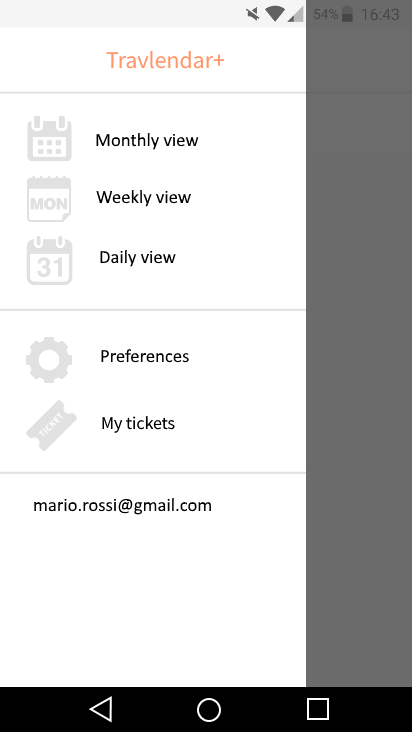
\includegraphics[width=0.50\textwidth]{Images/Mockup/LeftPanel.png}}%
		\caption{Menu}
	\end{minipage}
	\begin{minipage}[b]{0.65\textwidth}
		\makebox[\textwidth][c]{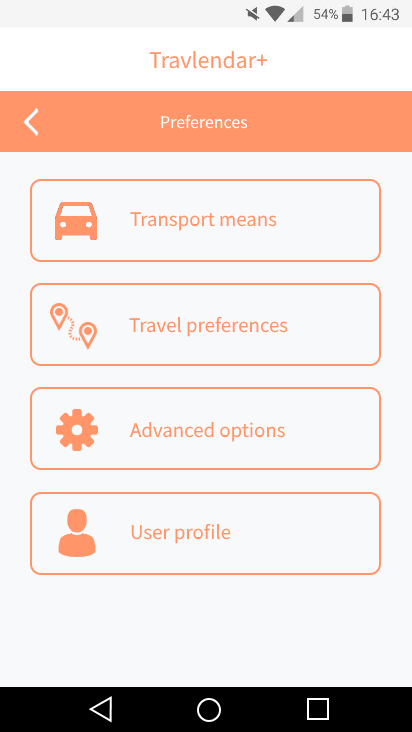
\includegraphics[width=0.50\textwidth]{Images/Mockup/PreferencesManager.png}}%
		\caption{Preferences menu}
	\end{minipage}
\end{figure}
\clearpage
\begin{figure}[!h]
	\centering
	\begin{minipage}[b]{0.65\textwidth}
		\makebox[\textwidth][c]{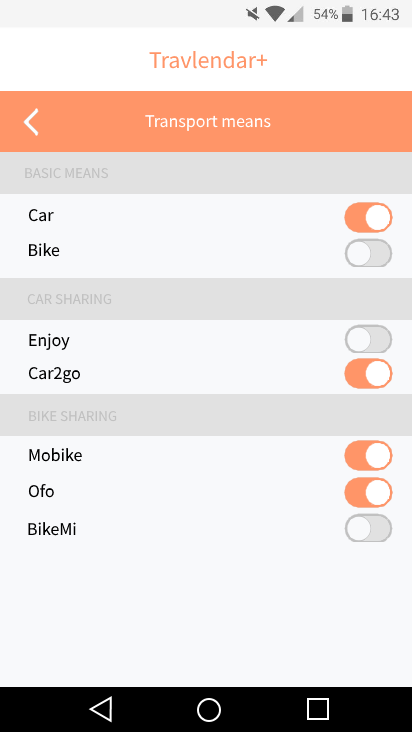
\includegraphics[width=0.50\textwidth]{Images/Mockup/transportMeansOpt.png}}%
		\caption{Transport means settings}
	\end{minipage}
	\begin{minipage}[b]{0.65\textwidth}
		\makebox[\textwidth][c]{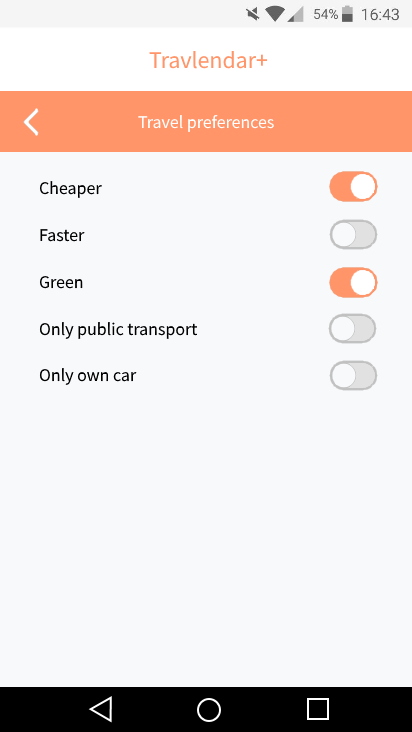
\includegraphics[width=0.50\textwidth]{Images/Mockup/TravelPreferences.png}}%
		\caption{Travel preferences}
	\end{minipage}
\end{figure}
\clearpage
\begin{figure}[!h]
	\centering
	\begin{minipage}[b]{0.65\textwidth}
		\makebox[\textwidth][c]{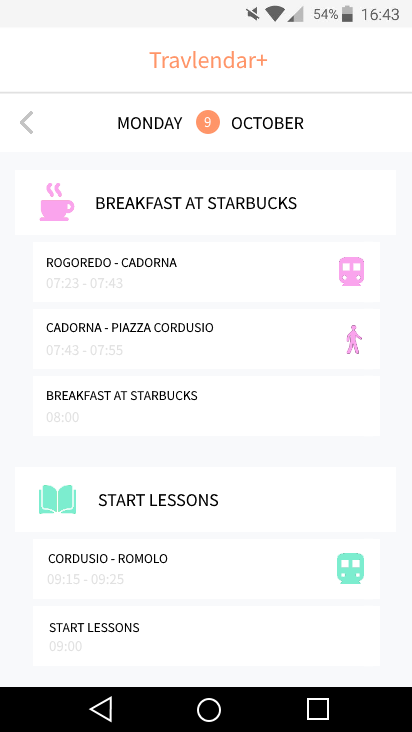
\includegraphics[width=0.50\textwidth]{Images/Mockup/DailySchedule.png}}%
		\caption{Daily schedule}
	\end{minipage}
	\begin{minipage}[b]{0.65\textwidth}
		\makebox[\textwidth][c]{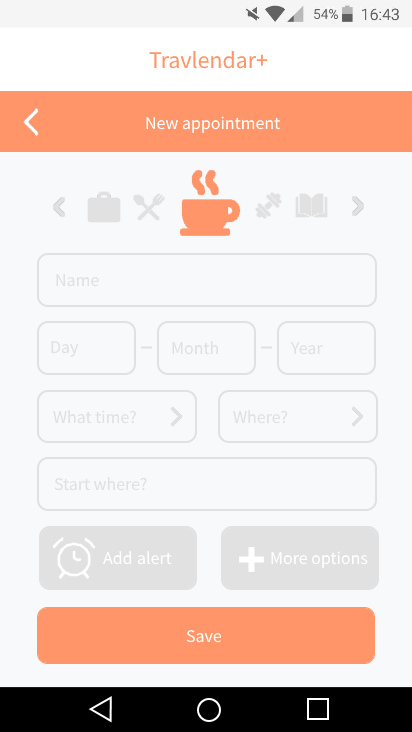
\includegraphics[width=0.50\textwidth]{Images/Mockup/EventCreator.png}}%
		\caption{New appointment}
	\end{minipage}
\end{figure}
\clearpage
\begin{figure}[!h]
	\centering
	\begin{minipage}[b]{0.65\textwidth}
		\makebox[\textwidth][c]{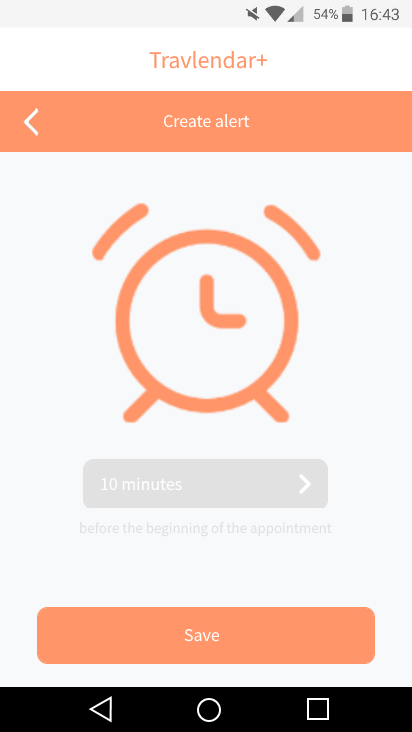
\includegraphics[width=0.50\textwidth]{Images/Mockup/AlarmCreator.png}}%
		\caption{New alert}
	\end{minipage}
	\begin{minipage}[b]{0.65\textwidth}
		\makebox[\textwidth][c]{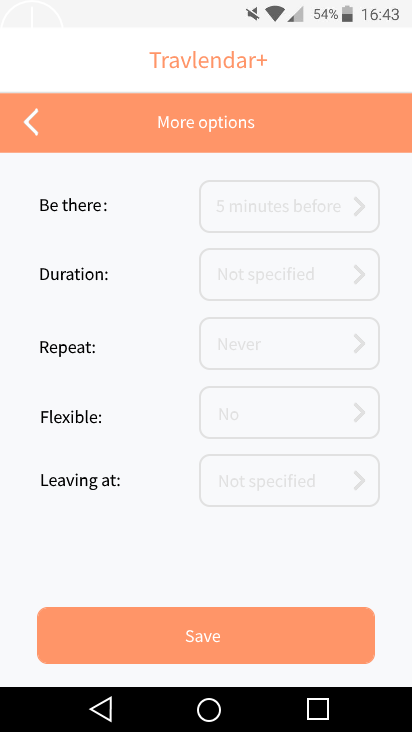
\includegraphics[width=0.50\textwidth]{Images/Mockup/OptionPanel.png}}%
		\caption{appointment options}
	\end{minipage}
\end{figure}
\clearpage
\begin{figure}[!h]
	\centering
	\begin{minipage}[b]{0.65\textwidth}
		\makebox[\textwidth][c]{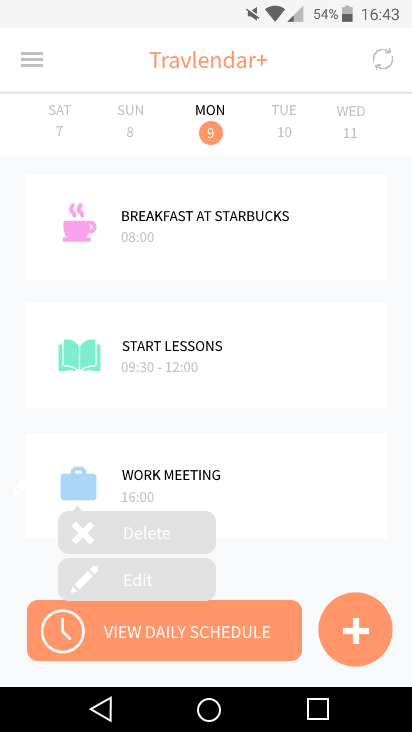
\includegraphics[width=0.50\textwidth]{Images/Mockup/BaseModificaDelete.png}}%
		\caption{Edit or delete appointment}
	\end{minipage}
	\begin{minipage}[b]{0.65\textwidth}
		\makebox[\textwidth][c]{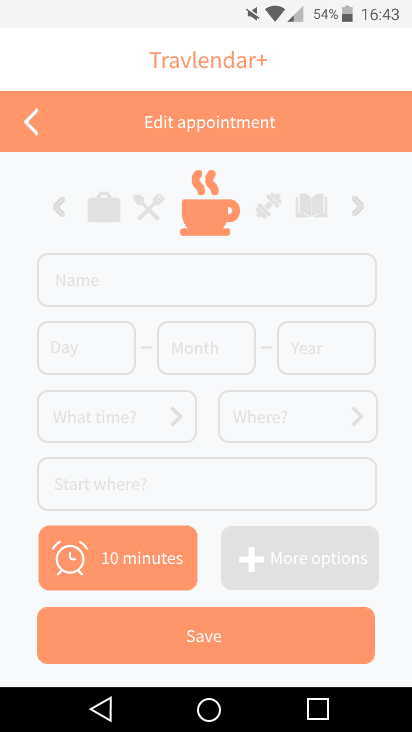
\includegraphics[width=0.50\textwidth]{Images/Mockup/EditAppointment.png}}%
		\caption{Edit appointment}
	\end{minipage}
\end{figure}
\clearpage
\begin{figure}[!h]
	\centering
	\begin{minipage}[b]{0.65\textwidth}
		\makebox[\textwidth][c]{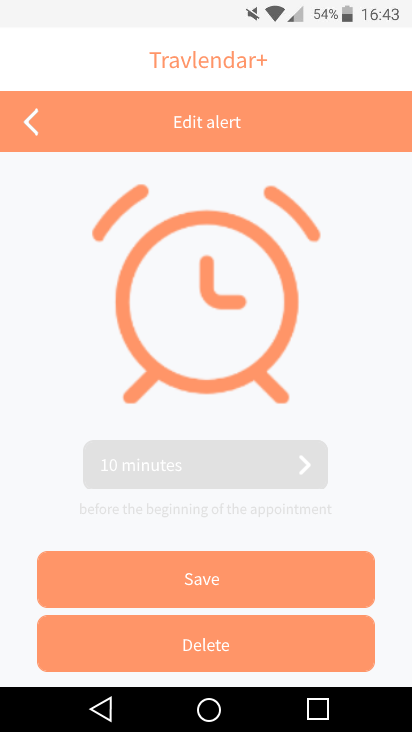
\includegraphics[width=0.50\textwidth]{Images/Mockup/AlarmEditDelete.png}}%
		\caption{Edit or delete alert}
	\end{minipage}
	\begin{minipage}[b]{0.65\textwidth}
		\makebox[\textwidth][c]{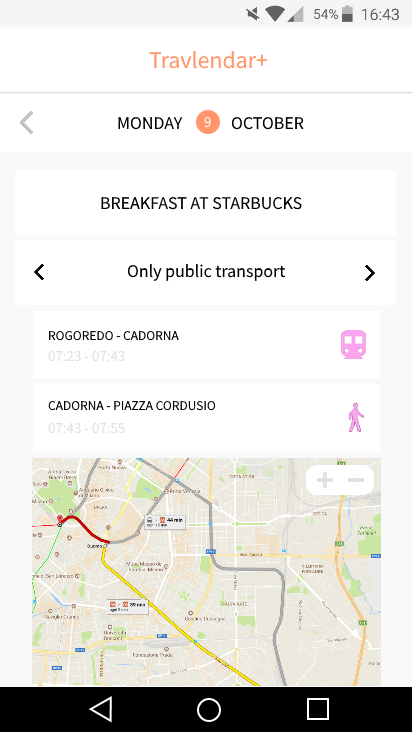
\includegraphics[width=0.50\textwidth]{Images/Mockup/TravelDetailsTrain.png}}%
		\caption{Travel details}
	\end{minipage}
\end{figure}
\clearpage
\begin{figure}[!h]
	\centering
	\begin{minipage}[b]{0.65\textwidth}
		\makebox[\textwidth][c]{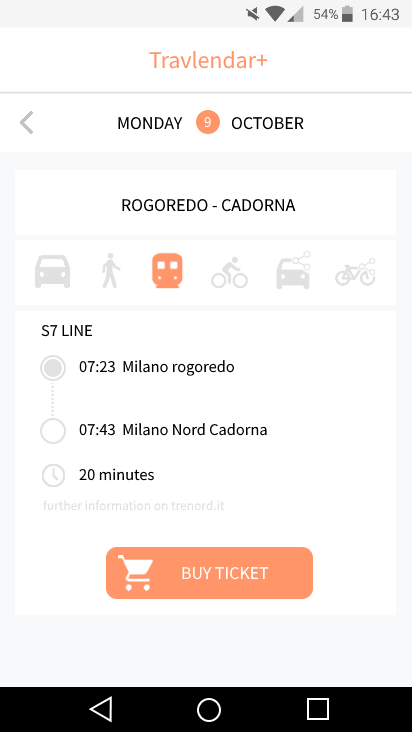
\includegraphics[width=0.50\textwidth]{Images/Mockup/MovementDetails.png}}%
		\caption{Movement details}
	\end{minipage}
\end{figure}
\clearpage

\subsubsection{Software interface}
The application makes uses of the following APIs:
\begin{itemize}
	\item Weather API: \href{url}{https://openweathermap.org/api}
	\item Google Maps API: \href{url}{https://developers.google.com/maps/}
	\item Trenord API: \href{url}{https://github.com/bluviolin/TrainMonitor/wiki/API-del-sistema-Viaggiatreno}
	\item Car2go API: \href{url}{https://github.com/car2go/openAPI}
	\item Enjoy API: \href{url}{https://github.com/mattiaongit/enjoy/blob/master/enjoy.py}
	\item BikeMi API: \href{url}{https://github.com/pierlauro/bikemi-unofficial-api}
	\item MoBike API: \href{url}{https://github.com/ubahnverleih/WoBike}
\end{itemize}
\subsection{Functional requirements}
\subsubsection{[G1] Allow a Guest to create a registered Travlendar+ account.}
\subsubsection{[G2] Allow an User to log in into his Travlendar+ account.}
\subsubsection{[G3] Allow an User to create a new appointment in his calendar.}
\begin{itemize}
	\item \textbf{[R9]} The user must be logged into the system to access application features.
	\item \textbf{[R10]} The system must be able to provide the user with an overview of his calendar and the user must be able to view all appointments fixed in a certain period.
	\item \textbf{[R11]} The user must be able to pick a chosen day from the overview of his calendar.
	\item \textbf{[R12]} The user must be able to choose the option of creating a new appointment.
	\item \textbf{[R13]} The system must ask the user to provide all information needed for the creation of a new appointment, such as place and time of start and overall duration.
	\item \textbf{[R14]} The system must check if an appointment overlaps with other events and must eventually notify it to the user.
	\item \textbf{[R15]} The user must confirm the creation of the new appointment.
	\item \textbf{[R16]} The system must save the user modifications in memory and the calendar must be updated.
	\item \textbf{[D2]} All information provided by the user in the process of appointment creation or modification must be formally corrected.
	
\end{itemize}
\subsubsection{[G4] Allow an User to delete an existing appointment from his calendar.}
\begin{itemize}
	\item \textbf{[R17]} The appointment intended to be modified must have been previously successfully created and not already deleted.
	\item \textbf{[R9]} The user must be logged into the system to access application features.
	\item \textbf{[R10]} The system must be able to provide the user with an overview of his calendar and the user must be able to view all appointments fixed in a certain period.
	\item \textbf{[R11]} The user must be able to pick a chosen day from the overview of his calendar.
	\item \textbf{[R18]} The user must be able to choose the option of deleting the appointment.
	\item \textbf{[R19]} The user must confirm the deletion.
	\item \textbf{[R20]} The system must remove a deleted appointment from the memory and cancel every alert related to it.
	\item \textbf{[R16]} The system must save the user modifications in memory and the calendar must be updated.
	\item \textbf{[R21]} Deleting process is not reversible.
	
\end{itemize}
\subsubsection{[G5] Allow an User to edit an existing appointment in his calendar.}
\begin{itemize}
	\item \textbf{[R17]} The appointment intended to be modified must have been previously successfully created and not already deleted.
	\item \textbf{[R9]} The user must be logged into the system to access application features.
	\item \textbf{[R10]} The system must be able to provide the user with an overview of his calendar and the user must be able to view all appointments fixed in a certain period.
	\item \textbf{[R22]} The user must be able to select a specific appointment in his calendar.
	\item \textbf{[R23]} The system must give the user access to all details of a selected appointment and the user must be allowed to edit the information needed.
	\item \textbf{[R14]} The system must check if an appointment overlaps with other events and must eventually notify it to the user.
	\item \textbf{[R24]} The user must confirm the modifications.
	\item \textbf{[R16]} The system must save the user modifications in memory and the calendar must be updated.
	\item \textbf{[D2]} All information provided by the user in the process of appointment creation or modification must be formally corrected.
	
\end{itemize}
\subsubsection{[G6] Allow an User to view his appointments.}
\begin{itemize}
	\item \textbf{[R9]} The user must be logged into the system to access application features.
	\item \textbf{[R10]} The system must be able to provide the user with an overview of his calendar and the user must be able to view all appointments fixed in a certain period.
	\item \textbf{[R25]} The user must be able to switch between different possible calendar, such as daily calendar, weekly calendar and monthly calendar.
	
\end{itemize}
\subsubsection{[G7] Allow an User to view his Daily Schedule}
\begin{itemize}
	\item \textbf{[R9]} The user must be logged into the system to access application features.
	\item \textbf{[R26]} The user must be able to select a specific day from his calendar.
	\item \textbf{[R27]} The system must be able to provide detailed information about the scheduled travels for a chosen day, showing the trace route and the estimated time required from each movement.
	\item \textbf{[R28]} The system must be able to choose a route between the possible travel alternatives according to the preferences expressed in the user profile settings and the information about external weather.
	\item \textbf{[D3]} Travel data are provided by an external agent.
	\item \textbf{[D4]} Information about weather are provided by an external agent.
	\item \textbf{[D5]} If the system displays a travel alternative, it means that it’s actually possible to successfully perform that travel in the way and in the time displayed.
	
\end{itemize}
\subsubsection{[G8] Allow an User to navigate and choose between different travel alternatives.}
\begin{itemize}
	\item \textbf{[R9]} The user must be logged into the system to access application features.
	\item \textbf{[R26]} The user must be able to select a specific day from his calendar.
	\item \textbf{[R27]} The user must be able to select a specific travel in the chosen day.
	\item \textbf{[R28]} The system must be able to provide the user with an overview of the possible travel alternatives for the chosen travel, specifying all details for each one.
	\item \textbf{[R29]} The user must be able to filter the travel alternatives furnished by the system according to defined parameters, such as time of travelling or overall cost.
	\item \textbf{[R30]} The user must be able to choose a favourite travel option different from the displayed default one.
	\item \textbf{[R31]} The system must update the daily schedule according to the travel option chosen by the user and the user must be able to see the new updated schedule.
	\item \textbf{[D5]} If the system displays a travel alternative, it means that it’s actually possible to successfully perform the travel in the way and in the time displayed.
	
\end{itemize}
\subsubsection{[G9] Allow an User to manage alerts for each appointment.}
\begin{itemize}
	\item \textbf{[R32]} The system must give the user the possibility of adding an alert to an appointment while it is being created or modified.
	\item \textbf{[R33]} The user must be able to choose a desired interval of time for the warning alert.
	\item \textbf{[R34]} The user must confirm the alert creation and the system must save the insertion in the memory.
	\item \textbf{[R35]} The user must be able to modify or remove the inserted alert when needed.
	\item \textbf{[R36]} In case of any alert modification made by the user, the user must confirm the modification and the system must save all changes.
	\item \textbf{[D6]} If a user creates a new alert, he must receive the notification after the specified amount of time.
	
\end{itemize}
\subsubsection{[G10] Allow an User to manage his travel preferences.}
\begin{itemize}
	\item \textbf{[R9]} The user must be logged into the system to access application features.
	\item \textbf{[R39]} The user must be able to access the preferences panel of his account.
	\item \textbf{[R40]} The system must give the user the possibility of setting various preferences, such as owned and preferred travel means, address of Home and other general travel preferences.
	\item \textbf{[R41]} The user must be able to edit the provided preferences when needed.
	
\end{itemize}
\subsubsection{[G11] Allow an User to buy public transportation tickets.}
\begin{itemize}
	\item \textbf{[R9]} The user must be already logged into the system to access his calendar.
	\item \textbf{[R26]} The user must be able to select a specific day from his calendar.
	\item \textbf{[R27]} The user must be able to select a specific travel in the chosen day.
	\item \textbf{[R37]} The system must give to the user the possibility of buying the ticket for the selected travel.
	\item \textbf{[R38]} The system must save a copy of the bought tickets and the user must be able to view them when needed.
	\item \textbf{[D7]} The payment process and ticket acquisition is made by an external public transport service.
\end{itemize}
\subsection{Design constraints}
\subsubsection{Standards compliance}
The application must require to the user different permissions:
\begin{itemize}
	\item Accesso to the calendar;
	\item Get hit position with GPS;
	\item Access to device storage.
\end{itemize}
\subsubsection{Hardware limitations}
The application, at the moment, runs only on Android 4.0.3 version or newer. \\
The device needs:
\begin{itemize}
	\item Internet connection;
	\item GPS;
	\item Space for save application in memory.
\end{itemize}
Actual devices on the market satisfy all these requirements.
\subsection{Software system attributes}
\subsubsection{Reliability}
The system must guarantee a 24/7 service.
\subsubsection{Availability}
The system requires a GPS service and internet connection in order to work properly. When the connection is down the system works with the last updated information available in the device memory. 
\subsubsection{Security}
The application must provide secure storage for all sensitive data inserted by the user. One way to achieve it is the use of cryptographical techniques.
\subsubsection{Maintainability}
The application now is in beta version, this means that can present some bugs. Certainly, the application will be periodically upgraded and each release allow to remove known bugs and add more functionality.
Periodically all information that are stored inside the application must be backed up, in order to reduce danger of lost information in case of malfunction of the application.
\subsubsection{Portability}
Now the application has been developed only for android device (more specifically only for android version 4.0.3 Ice Cream Sandwich or newer versions).
Further developments will lead this application also in iOS devices.
Another possible development is the creation of a web site that is synchronized with application, and allow to the user to control their appointment also on desktop pc and laptop.
